\documentclass{article}
\usepackage{amsthm,hyperref,mathtools,mathpartir,cleveref,mathrsfs,amssymb,url,paralist,xspace,braket,ifmtarg}
\usepackage[status=draft]{fixme}
\newtheorem{thm}{Theorem}[section]
\crefname{thm}{Theorem}{Theorems}
\newtheorem{lem}[thm]{Lemma}
\crefname{lem}{Lemma}{Lemmas}
\newtheorem{cor}[thm]{Corollary}
\crefname{cor}{Corollary}{Corollaries}
\theoremstyle{definition}
\newtheorem{defn}[thm]{Definition}
\crefname{defn}{Definition}{Definitions}
\newtheorem{defns}[thm]{Definitions}
\crefname{defns}{Definitions}{Definitions}
\newtheorem{eg}[thm]{Example}
\crefname{eg}{Example}{Examples}
\theoremstyle{remark}
\newtheorem{rmk}[thm]{Remark}
\crefname{rmk}{Remark}{Remarks}
\usepackage{tikz}
\usepackage{tikz-cd}
\usetikzlibrary{decorations.markings}
\tikzset{edge/.style={decoration={markings,mark=at position 0.5 with {\arrow{>}}},postaction={decorate}}}
\tikzset{vertex/.style={circle,draw,inner sep=1pt}}
\usetikzlibrary{shapes.geometric}
\tikzset{outer/.style={regular polygon,regular polygon sides=3,inner sep=1pt,draw,shape border rotate=180}}
\tikzset{houter/.style={regular polygon,regular polygon sides=3,inner sep=1pt,draw,shape border rotate=270}}
\tikzset{cross/.style={white,line width=3pt}}
\let\sto\looparrowright
\def\M{\mathcal{M}}
\def\C{\mathcal{C}}
\def\K{\mathcal{K}}
\def\P{\mathcal{P}}
\def\Q{\mathcal{Q}}
\def\D{\mathcal{D}}
\def\G{\mathcal{G}}
\def\H{\mathcal{H}}
\def\K{\mathcal{K}}
\def\L{\mathcal{L}}
% \def\Cat{\ensuremath{\mathcal{C}\mathit{at}}}
\let\setof\Set
\def\Set{\mathbf{Set}}
\def\Cat{\ensuremath{\mathbf{Cat}}}
\def\Fib{\mathcal{F}\mathit{ib}}
\def\Prof{\mathcal{P}\mathit{rof}}
\def\cpg{\ensuremath{\mathbf{CPG}}\xspace}
\def\dom{\mathrm{dom}}
\def\cod{\mathrm{cod}}
\def\id{\mathrm{id}}
\def\side#1{{\scriptstyle(#1)}}
\def\sid{\side{\id}}
% \def\twocell#1#2#3#4{\inferrule*[Left={$\side{#1}$},Right={$\side{#4}$}]{#2}{#3}}
% \def\twocelll#1#2#3#4{\inferrule*[left={$\side{#1}$},Right={$\side{#4}$}]{#2}{#3}}
% \def\twocellr#1#2#3#4{\inferrule*[Left={$\side{#1}$},right={$\side{#4}$}]{#2}{#3}}
% \def\twocelllr#1#2#3#4{\inferrule*[left={$\side{#1}$},right={$\side{#4}$}]{#2}{#3}}

\newcounter{nodemaker}
\setcounter{nodemaker}{0}
\def\twocell#1{%
  \global\edef\mynodeone{twocell\arabic{nodemaker}}%
  \stepcounter{nodemaker}%
  \global\edef\mynodetwo{twocell\arabic{nodemaker}}%
  \stepcounter{nodemaker}%
  \ar[#1,phantom,shift left=3,""{name=\mynodeone}]%
  \ar[#1,phantom,shift right=3,""'{name=\mynodetwo}]%
  \ar[Rightarrow,from=\mynodeone,to=\mynodetwo]%
}
\newcommand{\drpullback}[1][dr]{\ar[#1,phantom,near start,"\lrcorner"]}
\newcommand{\dlpullback}[1][dl]{\ar[#1,phantom,near start,"\llcorner"]}
\newcommand{\urpullback}[1][ur]{\ar[#1,phantom,near start,"\urcorner"]}
\newcommand{\ulpullback}[1][ul]{\ar[#1,phantom,near start,"\ulcorner"]}

\let\ot\leftarrow
\let\xto\xrightarrow
\let\xot\xleftarrow
\let\tot\leftrightarrow
\def\o{^{\circ}}
\def\type{\;\mathsf{type}}
\let\types\vdash
\tikzset{horiz/.style={"\mathclap\bullet" description}}
\def\genus{\mathsf{genus}}
\def\degree{\mathsf{degree}}
\def\rank{\mathsf{rank}}
\def\N{\mathbb{N}}
\def\Np{\N_{\bullet}}
\def\hy{\mathbf{HyGph}}
\def\thy{\mathcal{T}}
\def\dhy{\mathcal{D}}
\def\fhy{\mathcal{F}}
\def\ehy{\mathcal{E}\mathit{xt}\mathcal{H}\mathit{y}\mathcal{G}\mathit{ph}}

\makeatletter
\def\ins#1#2#3#4{#1 \underset{\@ifmtarg{#2}{#3}{#3\in #2}}{\circ} #4}
\def\insy{\circ}
\makeatother
\def\bE{\mathbf{E}}
\def\bC{\ensuremath{\mathbf{C}}\xspace}
\def\bS{\ensuremath{\mathbf{S}}\xspace}
\def\Ebar{\overline{\mathbf{E}}}
\def\Gbar{\overline{\mathcal{G}}}
\def\Cbar{\overline{\mathcal{C}}}
\def\Hbar{\overline{\mathcal{H}}}
\def\Kbar{\overline{\mathcal{K}}}
\def\Lbar{\overline{\mathcal{L}}}
\def\dhybar{\overline{\mathcal{D}}}

\hyphenation{hyper-graph}
\hyphenation{hyper-graphs}

\title{Hypercategories and some kind of type theory}
\author{Dan Licata \and\ Mitchell Riley \and\ Patrick Schultz \and\ Michael Shulman}
\begin{document}
\maketitle

\section{Hypergraphs}
\label{sec:hypergraphs}

The natural numbers $\N$ include zero.

\begin{defn}
  A \textbf{hypergraph} is a diagram of sets and functions
  \[ V \ot F \to E \xto{\genus} \N\]
  in which each fiber of the map $F\to V$ is a finite set equipped with a linear ordering.

  The elements of $E$ are called \textbf{edges}, those of $V$ are called \textbf{vertices}, and those of $F$ are called \textbf{flags}.
  If a vertex and an edge are the image of a common flag, we say they are \textbf{incident}; thus the flags are the ``witnesses of incidence''.
  We also speak of a flag as being \textbf{incident} to its associated edge and vertex.
\end{defn}

We allow vertices that are not incident to any edges, and edges that are not incident to any vertices.
Also a vertex and an edge can be ``incident more than once'', i.e.\ the image of more than one common flag.

\begin{defn}
  Let $\G=(V\ot F\to E\to\N)$ be a hypergraph.
  \begin{itemize}
  \item The \textbf{degree} of a vertex in $\G$ is the cardinality of the set of flags adjacent to it, which is a natural number.
    The \textbf{rank} of an edge in $\G$ is the cardinality of the set of flags adjacent to it, which in general can be finite or infinite.
    We say $\G$ has \textbf{finite rank} if all its ranks are finite, and $\G$ is \textbf{finite} if the sets $V$ and $E$ (hence also $F$) are finite.
  \item The set of \textbf{connected components} of $\G$ is the pushout of the span $V \leftarrow F \to E$.
    We say $\G$ is \textbf{connected} if it has exactly one connected component.
    % In particular, vertices not incident to any edges, and edges not incident to any vertices, lie in their own connected components.
  \item We say $\G$ has \textbf{genus zero} if all of its edges have genus zero.
  \item We say $\G$ is \textbf{simple} if no edge is incident to any vertex more than once, so that the span $E \ot F \to V$ is a relation.
  \end{itemize}
\end{defn}

The (directed) hypergraphs of~\cite{glpn:directed-hypergraphs} are our (directed) finite simple hypergraphs of genus zero, but without the orderings on the flags adjacent to each vertex.
\fxnote{Add some examples.}

\begin{defn}
  A \textbf{morphism of hypergraphs} is a diagram
  \[
  \begin{tikzcd}[row sep=tiny]
    V' \ar[dd] & F' \ar[dd] \ar[r] \ar[l] \dlpullback[ddl] & E' \ar[dr] \ar[dd]\\
    &&& \N\\
    V  & F \ar[r] \ar[l] & E \ar[ur]
  \end{tikzcd}
  \]
  in which the left-hand square is a pullback and preserves the linear orderings on the fibers.
  This defines the category $\hy$ of hypergraphs.
\end{defn}

Let $\Np$ be the set $\setof{(k,n) \in \N\times \N | k<n}$, with $\ell:\Np\to \N$ the second projection.
Thus the fiber of $\ell$ over $n\in\N$ is the canonical $n$-element linear order.
Let $P_\ell$ be the polynomial endofunctor of $\Set$ defined by $\ell$, i.e.\ the composite
\[ \Set \xto{(\Np)^*} \Set/\Np \xto{\Pi_\ell} \Set/\N \xto{\Sigma_\N} \Set.\]
Thus an element of $P_\ell(E)$ is a finite list of elements of $E$.

\begin{lem}
  The category $\hy$ of hypergraphs is equivalent to the comma category
  \[
  \begin{tikzcd}
    \hy \ar[rr] \ar[d] \twocell{drr} && \Set \ar[d,equals] \\
    \Set/\N \ar[r,"{\Sigma_\N}"'] & \Set \ar[r,"P_\ell"'] & \Set.
  \end{tikzcd}
  \]
\end{lem}
\begin{proof}
  An object of the comma category consists of a set $E$ with a map $E\to \N$, together with a set $V$ and a map $V \to P_\ell E$.
  By definition of $P_\ell$, the latter map is equivalent to a map $f:V\to \N$ together with a map $f^*\Np \to E$.
  And the set of maps $f:V\to\N$ is equivalent to the groupoid of maps $F\to V$ with finite linearly ordered fibers (via the equivalence $F=f^*\Np$), so this corresponds exactly to the above definition of a hypergraph.

  A morphism in the comma category consists of a map $E'\to E$ over $\N$ and a map $V'\to V$ making the evident square commute.
  The composite $V'\to V\to P_\ell E$ corresponds to precomposing the maps $V' \to V \to \N$, which means taking the pullback
  \[
  \begin{tikzcd}
    V' \ar[d] & F' \dlpullback \ar[d] \ar[l] \ar[dr] \\
    V & F \ar[l] \ar[r] & E
  \end{tikzcd}
  \]
  Whereas the composite $V' \to P_\ell E' \to P_\ell E$ corresponds to taking the composite
  \[
  \begin{tikzcd}
    V' & F' \ar[l] \ar[r] \ar[dr] & E' \ar[d] \\
    && E
  \end{tikzcd}
  \]
  Thus saying that they are equal reproduces exactly the above definition of hypergraph morphism.
\end{proof}

\begin{cor}
  $\hy$ is a presheaf topos.
  In particular, it is complete and cocomplete.
\end{cor}
\begin{proof}
  The functor $P_\ell \circ \Sigma_\N : \Set/\N \to \Set$ is polynomial, hence a parametric right adjoint.
  Thus, since $\Set/\N$ is a presheaf topos, by~\cite{cj:clfrag} the comma category $\hy$ is again a presheaf topos.
\end{proof}

In the comma category presentation, the terminal hypergraph $\thy$ has $E=\N$, with $\genus : E\to\N$ the identity, and $V = P_\ell E = P_\ell \N$ with $V\to P_\ell E$ the identity.
That is, there is exactly one edge of each genus, and for each finite list of such edges there is exactly one vertex adjacent to those edges in that order.

Various other kinds of hypergraphs can be defined as slice categories of $\hy$, which again form presheaf toposes since the slice of any presheaf topos is a presheaf topos.
For instance, if $\thy_0$ denotes the sub-hypergraph of $\thy$ containing only the edge of genus 0 and exactly the vertices that are adjacent only to that edge (of which there are $\N$), then $\hy/\thy_0$ is the category of genus-zero hypergraphs.

A little less trivially, let $\dhy$ denote the hypergraph with $E=\N$ (i.e.\ exactly one edge of each genus) and where the fiber of $V\to P_\ell E$ over a list of edges of length $n$ is the $(n+1)$-element linear order.
We think of the $k^{\mathrm{th}}$ element of this fiber as a vertex with its $n$ adjacent flags partitioned into the first $k$ elements and the last $n-k$ elements.

\begin{defn}
  The category of \textbf{directed hypergraphs} is the slice category $\hy/\dhy$.
\end{defn}

Thus, a directed hypergraph is a hypergraph in which at each vertex the list of adjacent flags is partitioned into two linear orders, which we call the \textbf{incoming} and \textbf{outgoing} flags respectively.
The numbers of incoming and outgoing flags are respectively called the \textbf{in-degree} and \textbf{out-degree} of the vertex.
Similarly, the \textbf{in-rank} and \textbf{out-rank} of an edge are respectively the cardinalities of the sets of outgoing (from their vertices, hence incoming to the edge) and incoming (to their vertices, hence outgoing from the edge) flags adjacent to it.

The unique projection $\dhy\to\thy$ has a section $\thy\to\dhy$ that chooses the $0^{\mathrm{th}}$ element of each fiber.
Thus, we have
\[\hy \simeq \hy/\thy \simeq (\hy/\dhy)/(\thy\to\dhy).\]
In other words, arbitrary hypergraphs can also be regarded as particular directed ones, namely those in which all flags are outgoing.
This is one advantage of hypergraphs over ordinary graphs.

\begin{defn}
  A directed hypergraph of genus zero is called a \textbf{polygraph}.
  In this case its edges are called \textbf{objects} and its vertices \textbf{morphisms}.
\end{defn}

A polygraph is the underlying data of a polycategory or a (colored) prop: each morphism has a finite list of ``source'' objects and a finite list of ``target'' objects.
%The category of polygraphs is equivalently the category of presheaves on the category with objects $0$ and $(m,n)$ for $m,n\in\mathbb{N}$ and $m+n$ distinct arrows $0\to (m,n)$.
Our graph-theoretic representation invokes the Poincar\'e dual ``string diagram convention'', in which objects are 1-dimensional and morphisms are 0-dimensional.
The category of polygraphs is the slice category $\hy/(\thy_0\times\dhy)$, hence again a presheaf topos.
The fact that we can define polygraphs in this way is another advantage of using hypergraphs; as we will see, it makes the notion of ``labeled graph'' very easy to define.

Other conditions on hypergraphs are not expressible as slices and do not define presheaf toposes.
For instance:

\begin{defn}
  A hypergraph is \textbf{rooted} if it is equipped with a specified vertex called the \textbf{root}.
\end{defn}

To express this categorically, for each vertex $v$ in $\thy$, let $\thy_v$ denote the sub-hypergraph of $\thy$ containing only $v$ and all the edges adjacent to it.
Then the category of rooted hypergraphs is the disjoint union of coslice categories $\coprod_v (\thy_v/\hy)$.
Thus it has connected limits and colimits, but not disconnected ones.

In general, we think of the root as ``not really there'' and the flags adjacent to it as ``free''.
In a directed rooted hypergraph, we think of the incoming or outgoing edges of the root as ``incoming/outgoing to the entire graph''.
For instance, given the graph on the left with $\ast$ the root:
\begin{equation}
  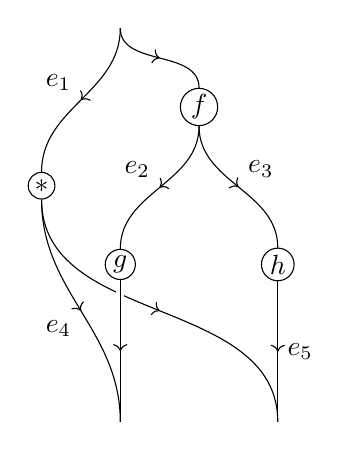
\begin{tikzpicture}
    \node[vertex] (r) at (0,0) {$\ast$};
    \node[vertex] (f) at (2,1) {$f$};
    \node[vertex] (g) at (1,-1) {$g$};
    \node[vertex] (h) at (3,-1) {$h$};
    \draw[edge] (1,2) to[out=-90,in=90] (f);
    \draw[edge] (1,2) to[out=-90,in=90] node[auto,swap] {$e_1$} (r);
    \draw[edge] (r) to[out=-90,in=90] (3,-3);
    \draw[edge] (h) to[out=-90,in=90] node[auto] {$e_5$} (3,-3);
    \draw[cross] (g) to[out=-90,in=90] (1,-3);
    \draw[edge] (g) to[out=-90,in=90] (1,-3);
    \draw[edge] (r) to[out=-90,in=90] node[auto,swap] {$e_4$} (1,-3);
    \draw[edge] (f) to[out=-90,in=90] node[auto,swap] {$e_2$} (g);
    \draw[edge] (f) to[out=-90,in=90] node[auto] {$e_3$} (h);
  \end{tikzpicture}
  \qquad
  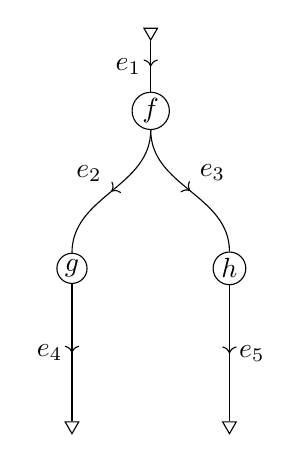
\begin{tikzpicture}
    \node[outer] (e1) at (2,2) {};
    \node[vertex] (f) at (2,1) {$f$};
    \node[vertex] (g) at (1,-1) {$g$};
    \node[vertex] (h) at (3,-1) {$h$};
    \node[outer] (e4) at (1,-3) {};
    \node[outer] (e5) at (3,-3) {};
    \draw[edge] (e1) to[out=-90,in=90] node[auto,swap] {$e_1$} (f);
    \draw[edge] (h) to[out=-90,in=90] node[auto] {$e_5$} (e5);
    \draw[edge] (g) to[out=-90,in=90] node[auto,swap] {$e_4$} (e4);
    \draw[edge] (f) to[out=-90,in=90] node[auto,swap] {$e_2$} (g);
    \draw[edge] (f) to[out=-90,in=90] node[auto] {$e_3$} (h);
  \end{tikzpicture}\label{eq:rooted-graph}
\end{equation}
we think of the edge $e_1$ as ``incoming to the graph'' and the edges $e_4,e_5$ as ``outgoing from the graph'', as drawn above on the right.

Note that an edge like $e_1$ that is ``incoming to the graph'' is \emph{incoming} to the root (as well as to other vertices like $f$), and one like $e_4$ or $e_5$ that is ``outgoing from the graph'' is \emph{outgoing} from the root (as well as from other vertices such as $g$ or $h$).
This choice, which as we will see makes the definition of insertion somewhat simpler, is only possible when using \emph{hyper}graphs, where edges can be incoming to multiple vertices and outgoing from multiple vertices.

% \begin{defn}\label{defn:loop}
%   A \textbf{loop} in a directed hypergraph is a sequence of flags
%   \[(f_0,g_0,f_1,g_1,\dots,f_n,g_n),\]
%   for $n\ge 0$, such that
%   \begin{enumerate}
%   \item Each $f_i,g_i$ are incident on the same edge, and
%   \item Each $g_i,f_{i+1}$ (including $g_n,f_0$ by mod-$n$ arithmetic) are incident on the same vertex, with $g_i$ incoming and $f_{i+1}$ outgoing.
%   \end{enumerate}
%   In particular, a loop with $n=0$ is an edge that is both incoming and outgoing to the same vertex.
%   A directed hypergraph is \textbf{loop-free} if it contains no loops.
% \end{defn}

% The left-hand rooted graph in~\eqref{eq:rooted-graph} is loop-free, which makes sense when considering the right-hand ``graph with free flags'' that it represents.
% If we chose to represent edges ``incoming to the graph'' by edges \emph{outgoing} to the root, then we would have to represent the right-hand ``graph with free flags'' in~\eqref{eq:rooted-graph} by the following rooted graph:
% \begin{equation}
%     \begin{tikzpicture}
%     \node[vertex] (r) at (0,0) {$\ast$};
%     \node[vertex] (f) at (2,1) {$f$};
%     \node[vertex] (g) at (1,-1) {$g$};
%     \node[vertex] (h) at (3,-1) {$h$};
%     \draw[edge] (r) to[out=90,in=90] node[auto] {$e_1$} (f);
%     \draw[edge] (h) to[out=-90,in=-90,looseness=2] node[auto] {$e_5$} (r);
%     \draw[edge] (g) to[out=-90,in=-90] node[auto,very near start] {$e_4$} (r);
%     \draw[edge] (f) to[out=-90,in=90] node[auto,swap] {$e_2$} (g);
%     \draw[edge] (f) to[out=-90,in=90] node[auto] {$e_3$} (h);
%   \end{tikzpicture}\label{eq:loop}
% \end{equation}
% which is not loop-free according to \cref{defn:loop} as written; thus we would have had to special-case the root vertex in \cref{defn:loop}.
% In fact, we regard~\eqref{eq:loop} as representing the following ``graph with free flags'':
% \begin{equation}
%   \begin{tikzpicture}
%     \node[vertex] (f) at (2,1) {$f$};
%     \node[vertex] (g) at (1,-1) {$g$};
%     \node[vertex] (h) at (3,-1) {$h$};
%     \draw[edge] (1,2) to[out=-90,in=90] (f);
%     \draw[edge] (1,2) to[out=-90,in=90] node[auto,swap,near end] {$e_1$} (-1,-4);
%     \draw[edge] (5,3) to[out=-90,in=90] node[auto] {$e_5$} (3,-3);
%     \draw[edge] (h) to[out=-90,in=90] (3,-3);
%     \draw[edge] (g) to[out=-90,in=90] (1,-3);
%     \draw[cross] (-1,3) to[out=-90,in=90] (1,-3);
%     \draw[edge] (-1,3) to[out=-90,in=90] node[auto,swap,near start] {$e_4$} (1,-3);
%     \draw[edge] (f) to[out=-90,in=90] node[auto,swap] {$e_2$} (g);
%     \draw[edge] (f) to[out=-90,in=90] node[auto] {$e_3$} (h);
%   \end{tikzpicture}\label{eq:loops2}
% \end{equation}
% in which $e_4$ and $e_5$ are ``incoming to the graph'' and $e_1$ is ``outgoing from the graph''.
% We do want to consider~\eqref{eq:loops2} as containing ``loops'', because there are paths from ``in'' to ``out'' that travel some paths ``backwards''.\fxnote{Is that right?}

Note also that we allow edges that are not adjacent to any vertices, or that are adjacent to only one vertex, but are \emph{not} adjacent to the root and hence not ``incoming'' or ``outgoing'' to the graph.
The following example shows a number of distinct degenerate possibilities in a directed hypergraph (where $\ast$ is the root):
\begin{center}
  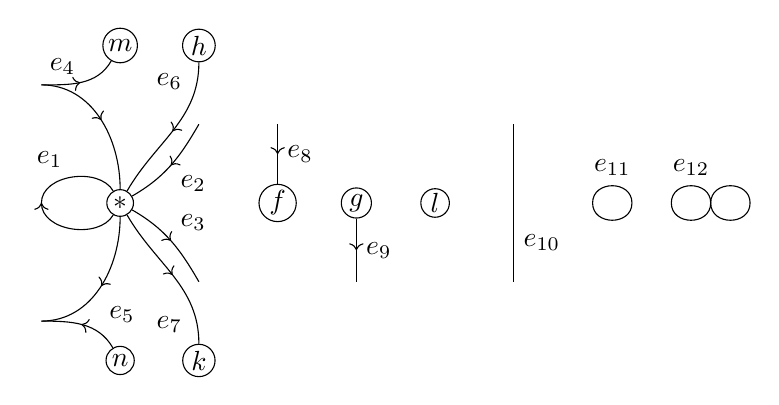
\begin{tikzpicture}
    \node[vertex] (r) at (0,0) {$\ast$};
    \draw[edge] (r) to[out=-120,in=-90] +(-1,0) to[out=90,in=120] node[auto] {$e_1$} (r);
    \draw[edge] (1,1) to[out=-120,in=30] node[auto] {$e_2$} (r);
    \draw[edge] (r) to[out=-30,in=120] node[auto] {$e_3$} (1,-1);
    \node[vertex] (h) at (1,2) {$h$};
    \draw[edge] (h) to[out=-90,in=60] node[auto,swap,near start] {$e_6$} (r);
    \node[vertex] (k) at (1,-2) {$k$};
    \draw[edge] (r) to[out=-60,in=90] node[auto,swap,near end] {$e_7$} (k);
    \node[vertex] (m) at (0,2) {$m$};
    \draw[edge] (-1,1.5) to[out=0,in=-120] node[auto,near start] {$e_4$} (m);
    \draw[edge] (-1,1.5) to[out=0,in=90] (r);
    \node[vertex] (n) at (0,-2) {$n$};
    \draw[edge] (n) to[out=120,in=0] node[auto,swap,near start] {$e_5$} (-1,-1.5);
    \draw[edge] (r) to[out=-90,in=0] (-1,-1.5);
    \node[vertex] (f) at (2,0) {$f$};
    \draw[edge] (2,1) -- node[auto] {$e_8$} (f);
    \node[vertex] (g) at (3,0) {$g$};
    \draw[edge] (g) -- node[auto] {$e_9$} +(0,-1);
    \node[vertex] (l) at (4,0) {$l$};
    \draw (5,1) -- node[auto,near end] {$e_{10}$} (5,-1);
    \draw (6.5,0) to[out=90,in=90,looseness=1.5] node[auto,swap] {$e_{11}$} (6,0) to[out=-90,in=-90,looseness=1.5] (6.5,0);
    \draw (7.5,0) to[out=90,in=90,looseness=1.5] node[auto,swap] {$e_{12}$} (7,0) to[out=-90,in=-90,looseness=1.5] (7.5,0);
    \draw (7.5,0) to[out=90,in=90,looseness=1.5] (8,0) to[out=-90,in=-90,looseness=1.5] (7.5,0);
  \end{tikzpicture}
\end{center}
Here $e_{10}$, $e_{11}$, and $e_{12}$ are all edges not adjacent to any vertices, with genera 0, 1, and 2 respectively.
We did not draw any arrows on them because only flags, not edges, are directed as ``incoming'' or ``outgoing''.
When interpreted as incoming or outgoing to the entire graph, the edges $e_1$--$e_7$ adjacent to the root above would be drawn as follows (preserving the ordering on incoming and outgoing edges to the root by drawing the incoming and outgoing edges to the graph in the same order).
\begin{center}
  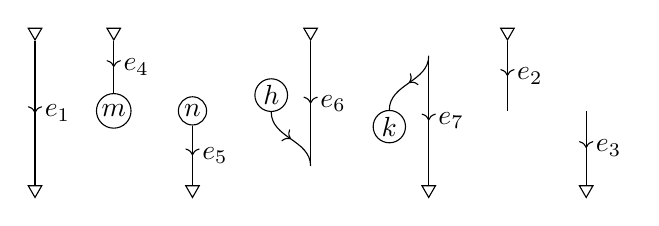
\begin{tikzpicture}
    \node[outer] (e1a) at (2,1) {};
    \node[outer] (e1b) at (2,-1) {};
    \draw[edge] (e1a) -- node[auto] {$e_1$} (e1b);
    \node[outer] (e2) at (8,1) {};
    \draw[edge] (e2) -- node[auto] {$e_2$} (8,0);
    \node[outer] (e3) at (9,-1) {};
    \draw[edge] (9,0) -- node[auto] {$e_3$} (e3);
    \node[vertex] (m) at (3,0) {$m$};
    \node[outer] (e4) at (3,1) {};
    \draw[edge] (e4) -- node[auto] {$e_4$} (m);
    \node[vertex] (n) at (4,0) {$n$};
    \node[outer] (e5) at (4,-1) {};
    \draw[edge] (n) -- node[auto] {$e_5$} (e5);
    \node[vertex] (h) at (5,.2) {$h$};
    \node[outer] (e6) at (5.5,1) {};
    \draw[edge] (e6) -- node[auto] {$e_6$} (5.5,-.7);
    \draw[edge] (h) to[out=-90,in=90]  (5.5,-.7);
    \node[vertex] (k) at (6.5,-.2) {$k$};
    \node[outer] (e7) at (7,-1) {};
    \draw[edge] (7,.7) -- node[auto] {$e_7$} (e7);
    \draw[edge] (7,.7) to[out=-90,in=90] (k);
  \end{tikzpicture}
\end{center}

We note that there are many ways in which a hypergraph can have nontrivial automorphisms.
One simple example is the graph with two vertices and no edges:
\begin{center}
\begin{tikzpicture}
  \node[circle,fill,inner sep=1pt] at (0,0) {};
  \node[circle,fill,inner sep=1pt] at (1,0) {};
\end{tikzpicture}
\end{center}
in which the two vertices can be swapped by an automorphism.
However, it is not necessary to be disconnected to have nontrivial automorphisms:
\begin{center}
  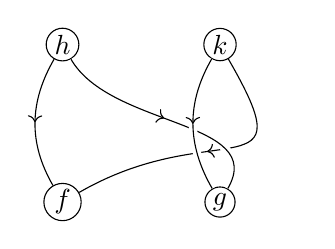
\begin{tikzpicture}[scale=2]
    \node[vertex] (f) at (0,0) {$f$};
    \node[vertex] (g) at (1,0) {$g$};
    \node[vertex] (h) at (0,1) {$h$};
    \node[vertex] (k) at (1,1) {$k$};
    \draw[edge] (h) to[out=-120,in=120] (f);
    \draw[edge] (k) to[out=-60,in=30,looseness=2] (f);
    \draw[cross] (h) to[out=-60,in=60] (g);
    \draw[edge] (h) to[out=-60,in=60] (g);
    \draw[cross] (k) to[out=-120,in=120] (g);
    \draw[edge] (k) to[out=-120,in=120] (g);
  \end{tikzpicture}
\end{center}
Here there is an automorphism that swaps $f$ with $g$ and swaps $h$ with $k$.
Moreover, if we orient this graph by giving the edges the left-to-right ordering in the picture, then this automorphism preserves the orientation.
This example cannot be rooted (the automorphism has no fixed points) --- or more precisely, it cannot occur in the connected component of the root --- but if we use edges that are incident on more than two vertices then we can have nontrivial automorphisms with fixed points:
\begin{center}
  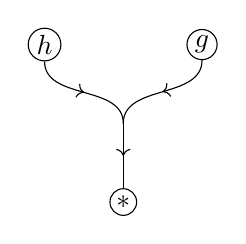
\begin{tikzpicture}
    \node[vertex] (f) at (0,0) {$\ast$};
    \node[vertex] (g) at (1,2) {$g$};
    \node[vertex] (h) at (-1,2) {$h$};
    \draw[edge] (g) to[out=-90,in=90] (0,1);
    \draw[edge] (h) to[out=-90,in=90] (0,1);
    \draw[edge] (0,1) -- (f);
  \end{tikzpicture}
\end{center}
Here there is an automorphism that swaps $g$ and $h$ and fixes the root $\ast$.
The most restrictive thing we can say about about automorphisms is:

\begin{lem}
  A connected rooted directed binary hypergraph has no nontrivial automorphisms.
\end{lem}
\begin{proof}
  Suppose $\phi$ is an automorphism.
  By assumption, it must preserve the root.
  Since it is locally-ordered, it must preserve all edges adjacent to the root.
  But since each of those edges is adjacent to exactly one other vertex, it must preserve those vertices too.
  Proceeding inductively we find that it must preserve all edges and vertices in the connected component of the root, which is all of them since the graph is connected.
\end{proof}

The presence of nontrivial automorphisms means that in general, we cannot simply ``pass to isomorphism classes'' of hypergraphs, and thus structures over hypergraphs are not definable using ``set-based shapes'', such as polynomial monads on the category of polygraphs.
In~\cite{bb:htapm} isomorphism classes and polynomial monads are shown to work for certain subclasses of graphs, but even there such a restriction is technical and error-prone.
Thus, we will generally work instead with categories and groupoids, never passing to isomorphism classes, and using a pseudomonad rather than a strict one.

We end this section by comparing our graphs to others in the literature.
Graphs with ``free flags'' have been used in defining many kinds of operads, but usually only in a ``non-hyper'' version, corresponding to non-cartesian operads.
The corresponding restriction in our theory is the following:

\begin{defn}
  A hypergraph is \textbf{binary}, or simply a \textbf{graph}, if % for each edge $e$ we have
  % \[ \rank(e) + 2 \cdot \genus(e)  = 2, \]
  % i.e.\ if
  every edge either has rank 2 and genus 0, or rank 0 and genus 1.
\end{defn}

This condition is not naturally expressible in terms of the category $\hy$, since the morphisms in $\hy$ do not preserve ranks of edges.
Amusingly, however, it can be reformulated by saying that the rank of an edge is the same as its ``Euler characteristic'' $\chi=2-2g$.

In a binary rooted hypergraph, we can define an involution on the set of flags not adjacent to the root by sending each flag to the other flag of its corresponding edge, if that flag is not adjacent to the root, or to itself otherwise.
The quotient of this involution is then isomorphic to the set of edges that are adjacent to some non-root vertex.
Thus, we can equivalently define a binary rooted hypergraph by giving
\begin{itemize}
\item a set $F$ of flags (the flags not adjacent to the root),
\item an involution on $F$,
\item a set of ``exceptional linear edges'' (the edges adjacent to the root twice),
\item a set of ``exceptional loops'' (the edges not adjacent to any vertex --- the only ones with genus 1), and
\item a set $V$ of (non-root) vertices and a function $F\to V$ with finite linearly ordered fibers (equivalently, a ``partition'' of $F$ into finite linearly ordered blocks, some of which are allowed to be empty).
\end{itemize}
This is the definition of ``graph'' used commonly in operad theory, e.g.~\cite{bm:gen-opds,km:gwcqceg,costello:ainf,mms:wheeled-props,gk:modular-operads}, although often exceptional loops and edges are omitted or treated inconsistently.

Alternatively, if we remove the root but not the flags adjacent to it, then the function $F\to V$ becomes a partial function, which is defined on a flag just when that flag is not adjacent to the root.
Now we still have the exceptional edges (those adjacent to two flags that are not adjacent to any vertices) and the exceptional loops (those not adjacent to any flags).
This is essentially how binary rooted hypegraphs are encoded in~\cite{bb:htapm}, except that their exceptional loops are ``adjacent to a single flag twice'' rather than to no flags at all.

Another possibility is to express the partial function $F\rightharpoonup V$ as a relation, i.e.\ a span $F \ot H \to V$ in which $H\to F$ is injective.
If we exclude the possibility of exceptional loops, then the function $F\to E$ is a 2-to-1 surjection and hence can be encoded up to isomorphism by a fixed-point-free involution of $F$.
This is the definition of graph from~\cite{jk:feynman} (though they call the elements $H$ the ``flags'' and those of $F$ the ``(directed) edges'').
TODO: Morphisms

Our convention about the orientations of flags adjacent to the root, though convenient for insertion, does mean that in the binary case such edges appear different from ordinary ones, since 

\begin{defn}
  A \textbf{directed rooted binary hypergraph} is a hypergraph that is separately directed, rooted, and binary, and moreover if we switched the direction of all flags adjacent to the root, then every edge would have equal in-rank and out-rank.
\end{defn}


\section{Insertion of hypergraphs}
\label{sec:insertion}

We now define an operation of \emph{insertion} of hypergraphs, which replaces some of the vertices in one graph by entire new graphs having the same ``flag structure''.
Suppose $\G = (V\ot F \to E\to \N)$ is a hypergraph, and for some subset $V_0 \subseteq V$ and each $v\in V_0$ we have a rooted hypergraph $\H_v = (V_v \ot F_v \to E_v\to \N)$ whose root $\ast_v$ has the same degree as $v$.
In the directed case, we require it to have the same in-degree and out-degree separately.
(Usually, $V_0$ will be either a single vertex or the set of all non-root vertices.)
There is a unique induced order-preserving (and, in the directed case, direction-preserving) bijection between the flags adjacent to $v$ and the flags adjacent to $\ast_v$, yielding a pair of pullback squares
\[
\begin{tikzcd}
  F \ar[d] & F_0 \ar[l] \dlpullback \ar[d] \ar[r] \drpullback & \sum_v F_v \ar[d]\\
  V & V_0 \ar[l] \ar[r] & \sum_v V_v
\end{tikzcd}
\]
where the map $V_0 \to \sum_v V_v$ sends $v$ to $\ast_v$.

We define the \textbf{insertion} of the $\H_v$'s into $\G$ at the vertices $v\in V_0$, denoted 
\[ \ins{\G}{V_0}{v}{\H_v} \]
to have an underlying span obtained by first taking the pushout of the following spans:
\[
\begin{tikzcd}
  E & F_0 \ar[d,equals] \ar[r] \ar[l] & \sum_v E_v & E' & E' \ar[l,equals]  \\
  F \ar[d] \ar[u] & F_0 \ar[l] \dlpullback \ar[d] \ar[r] \drpullback & \sum_v F_v \ar[d] \ar[u] &
  F' \ar[u] \ar[d] & F' \setminus F_0 \ar[l] \ar[d] \ar[u] \dlpullback \\
  V & V_0 \ar[l] \ar[r] & \sum_v V_v & V' & V' \setminus V_0 \ar[l]
\end{tikzcd}
\]
and then removing all the vertices coming from $V_0$ and the flags adjacent to them (those in $F_0$), as shown by the pullback on the right above.
Explicitly, this means:
\begin{itemize}
\item A vertex in $V'$ is either a non-root vertex of some $V_v$, or a vertex in $V\setminus V_0$.
\item A flag in $F'$ is either a flag in some $F_v$ not adjacent to the root, or a flag in $F$ not adjacent to a vertex in $V_0$.
  % Because $\mathbf{Set}$ is an adhesive category~\cite{ls:adhesive},
  The flags adjacent to a vertex coming from $V_v$ or $V$ are precisely those adjacent to it in $F_v$ or $F$ respectively.
  % In particular, the insertion hypergraph is naturally locally-ordered and directed if the inputs are.
\item An edge in $E'$ is either an edge in some $E_v$ or an edge in $E$, where an edge in $E_v$ adjacent to the root $\ast_v$ is identified with the corresponding edge adjacent to $v$ in $E$.
\end{itemize}
This relation on the edges that we quotient by is not an equivalence relation, so it may ``collapse homotopical information''.
We record this lost information in the induced genus function $E'\to \N$.
Specifically, we consider the commuting fork
\[
\begin{tikzcd}
F_0 \ar[r,shift left]\ar[r,shift right] & E + \sum_v E_v  \ar[r] & E' 
\end{tikzcd}
\]
as assigning to each $e\in E'$ a directed graph, whose set of vertices is its preimage in $E+\sum_v E_v$ and whose set of edges is its preimage in $F_0$.
This graph has a ``genus'', i.e.\ the rank of its fundamental group, and we define $\genus(e)$ to be this the sum of this genus and all the genera of its preimages in $E$ and $\sum_v E_v$.
\fxnote{Add some examples.}

The pushout in the definition of insertion is \emph{almost} a colimit construction in $\hy$.
If we define $\G_0$ to be the hypergraph $V_0 \ot F_0 \to F_0 \to \N$, then we have an inclusion map $\G_0\to \G$, and the above pushout of spans looks like it should be the pushout of this inclusion along a map $\G_0\to \sum_v \H_v$.

The problem is that there is no such map $\G_0\to \sum_v \H_v$, since the map on edges $F_0 \to \sum_v E_v$ will not generally preserve genera.
We can solve this problem by introducing the following more homotopical perspective on genera.

\begin{defn}
  An \textbf{extended hypergraph} is a span
  \[ V \ot F \to \bE \]
  in which $V$ and $F$ are sets, each fiber of the map $F\to V$ is a finite set equipped with a linear ordering, and $\bE$ is a groupoid.
  A \textbf{morphism of extended hypergraphs} is a diagram
  \[
  \begin{tikzcd}
    V' \ar[d] & F' \ar[d] \ar[r] \ar[l] \dlpullback[dl] \ar[dr,phantom,"\cong"] & \bE' \ar[d]\\
    V  & F \ar[r] \ar[l] & \bE
  \end{tikzcd}
  \]
  in which the left-hand square is a pullback and preserves the linear orderings on the fibers, and the right-hand square commutes up to a specified isomorphism.
  A \textbf{2-cell of extended hypergraphs} is a transformation between the two functors $\bE'\rightrightarrows \bE$ that commutes with the above isomorphisms.
  This defines the 2-category $\ehy$ of extended hypergraphs.
\end{defn}

We regard a hypergraph $\G$ as an extended hypergraph $\Gbar$ by replacing the set $E$ by the groupoid $\Ebar = \sum_{e\in E} \mathbf{B F}_{\genus(e)}$, the disjoint union over $e\in E$ of (the one-object groupoids corresponding to) the free groups of rank $\genus(e)$.
A function $E'\to E$ commuting with genera induces a functor $\Ebar' \to \Ebar$ that is an isomorphism on each free group; this defines a functor $\hy \to \ehy$ that is ``faithful'' in the sense that each functor $\hy(\G,\H) \to \ehy(\Gbar,\Hbar)$ is injective on isomorphism classes, though it is not in general full or essentially surjective.

An extended hypergraph is equivalent to one of the form $\Gbar$ just when its groupoid of edges is equivalent to a disjoint union of finitely generated free groups, in which case the corresponding set of edges is its set of connected components and the genera are the free ranks.
Extended hypergraphs of this sort are not generally closed under colimits, but they are closed under the particular colimits we are interested in.

Specifically, in the situation of an insertion, let $\Gbar$ and $\Hbar_v$ be the extended hypergraphs corresponding to $G$ and $H_v$ as above, and let $\Gbar_0$ be the extended hypergraph $V_0 \ot F_0 \to F_0$ with a \emph{discrete} groupoid of edges, i.e.\ where each edge has genus zero.
Then we do have morphisms of extended hypergraphs $\Gbar_0 \to \Gbar$ and $\Gbar_0 \to \sum_v \Hbar_v$, and we have:

\begin{thm}
  The extended hypergraph $\overline{\ins{\G}{V_0}{v}{\H_v}}$ corresponding to an insertion is equivalent to the subobject of the pseudo-pushout of $\Gbar_0 \to \Gbar$ and $\Gbar_0 \to \sum_v \Hbar_v$ in $\ehy$ determined by the vertices $V' \setminus V_0$.
\end{thm}
\begin{proof}
  This pseudo-pushout is obtained by taking the pushouts of the spans of vertices and flags and the pseudo-pushout of the groupoids of edges, and the connected components functor takes pseudo-pushouts of groupoids to pushouts of sets.
  Thus, it remains to show that each component of the pseudo-pushout of edge groupoids is a free group of the appropriate rank.
  But this follows from the ``van Kampen theorem for groupoids''.
\end{proof}

This makes it easy to show that insertion of hypergraphs is coherently associative in an appropriate sense.

\begin{thm}\label{thm:ins-assoc}
  Suppose we have
  \begin{itemize}
  \item a hypergraph $\G$,
  \item a subset $V_0$ of vertices in $\G$,
  \item for each $v\in V_0$ a rooted hypergraph $\H_v$ whose root $\ast_v$ has the same degree as $v$,
  \item for each $v$ a subset $W_v$ of non-root vertices in $\H_v$, and
  \item for each $v$ and $w\in W_v$ a rooted hypergraph $\K_w$ whose root $\ast_w$ has the same degree as $w$.
  \end{itemize}
  Then there is an isomorphism
  \begin{equation}
    \ins{\Bigl(\ins{\G}{V_0}{v}{\H_v}\Bigr)}{\sum_v W_v}{w}{\K_w} \;\cong \;
    \ins{\G}{V_0}{v}{\Bigl(\ins{\H_v}{W_v}{w}{\K_w}\Bigr)}\label{eq:ins-assoc}
  \end{equation}
  If moreover we also have
  \begin{itemize}
  \item for each $v$ and $w$ a subset $U_w$ of non-root vertices in $\K_w$, and
  \item For each $v,w$ and $u\in U_w$ a rooted hypergraph $\L_u$ whose root $\ast_u$ has the same degree as $u$,
  \end{itemize}
  then the following pentagon commutes:
  \[
  \begin{tikzcd}
    ((\G \insy \H_v)\insy \K_w)\insy \L_u \ar[rr,"\cong"] \ar[d,"\cong"'] &&
    (\G \insy (\H_v\insy \K_w))\insy \L_u \ar[d,"\cong"] \\
    (\G\insy \H_v) \insy (\K_w \insy \L_u) \ar[dr,"\cong"'] && \G\insy ((\H_v \insy \K_w) \insy \L_u) \ar[dl,"\cong"]\\
    & \G \insy (\H_v \insy (\K_w \insy \L_u))
  \end{tikzcd}
  \]
\end{thm}
\begin{proof}
  It is straightforward to see that when constructing iterated insertions of this sort, we can take all the pushouts at once and then remove the appropriate vertices and their associated flags.
  Since coproducts preserve pseudo-colimits, the pushouts involved in determining both sides of~\eqref{eq:ins-assoc} are equivalent to the pseudo-colimit in $\ehy$ of the diagram
  \[
  \begin{tikzcd}
    & \Gbar_0 \ar[dl] \ar[dr] & & \sum_v \Hbar_{v,0} \ar[dr] \ar[dl]\\
    \Gbar && \sum_v \Hbar_v  && \sum_v\sum_w \Kbar_w
  \end{tikzcd}
  \]
  hence equivalent, and thus isomorphic since they are discrete.
  The corresponding subobjects coincide since we are removing the same vertices $V_0 \cup (\bigcup_v W_v)$ on both sides.
  Similarly, the pushouts involved in all vertices of the pentagon are equivalent to the pseudo-colimit of the diagram
  \[
  \begin{tikzcd}[column sep=tiny]
    & \Gbar_0 \ar[dl] \ar[dr] & & \sum_v \Hbar_{v,0} \ar[dr] \ar[dl] && \sum_v\sum_w \Kbar_{w,0} \ar[dl]\ar[dr]\\
    \Gbar && \sum_v \Hbar_v  && \sum_v\sum_w\Kbar_w && \sum_v \sum_w \sum_u \Lbar_u
  \end{tikzcd}
  \]
  These equivalences commute up to isomorphism with the maps in the pentagon, so that the pentagon commutes up to isomorphism, and hence on the nose since all objects in it are discrete.
\end{proof}

Similarly, insertion is unital in an appropriate sense.
Let $\C_n$ denote the rooted $n$-corolla, which has $n$ edges of genus 0 and two vertices $c$ and $\ast$ (the root) each adjacent to all of them in the same order.

\begin{thm}\label{thm:ins-unit}
  If $\G$ is any hypergraph with a subset $V_0$ of vertices, then
  \[ \ins{\G}{V_0}{v}{\C_{\degree(v)}} \;\cong\; \G.\]
  Similarly, if $\G$ is any rooted hypergraph whose root has degree $n$, then
  \[ \ins{\C_n}{}{c}{\G} \;\cong\; \G. \]
  Finally, if $\G$ is any hypergraph with a subset $V_0$ of vertices, and for each $v\in V_0$ we have a rooted hypergraph $\H_v$ whose root has the same degree as $v$, then the following triangle commutes:
  \[
  \begin{tikzcd}
    (\G \insy \C_{\degree(v)} ) \insy \H_v \ar[rr,"\cong"] \ar[dr,"\cong"'] &&
    \G \insy (\C_{\degree(v)} \insy \H_v) \ar[dl,"\cong"] \\
    & \G \insy \H_v
  \end{tikzcd}
  \]
\end{thm}
\begin{proof}
  The pushout appearing in the insertion $\ins{\G}{V_0}{v}{\C_{\degree(v)}}$ adds a new copy of each vertex in $V_0$, connected to the same edges in the same order.
  The map $F_0 \to \sum_v \C_{\degree(v)}$ is an isomorphism, so no new edges are added and no genera are changed.
  Then we remove the old vertices in $V_0$, giving a result clearly isomorphic to the original $\G$.

  Similarly, the pushout in $\ins{\C_n}{}{c}{\G}$ adds a new copy of the root of $\G$, connected to the same edges in the same order.
  In this case it is $F_0 \to E$ that is an isomorphism, so no new edges are added and no genera are changed.
  Then we remove the old root, yielding a result isomorphic to $\G$.

  Finally, the associativity isomorphism in the triangle comes from identifying both sides with the pseudo-colimit of
  \[
  \begin{tikzcd}
    & \Gbar_0 \ar[dl] \ar[dr] & & \sum_v \Cbar_{\degree(v),0} \ar[dr] \ar[dl]\\
    \Gbar && \sum_v \Cbar_{\degree(v)}  && \sum_v \Hbar_v
  \end{tikzcd}
  \]
  Here the two inclusions $\Gbar_0 \to \sum_v \Cbar_{\degree(v)}$ and $\sum_v \Cbar_{\degree(v),0} \to \sum_v \Cbar_{\degree(v)}$ are actually a coproduct diagram on vertices, so that the vertices of the pseudo-colimit are the disjoint union of those in $\G$ and those in $\sum_v \H_v$.
  The left-hand diagonal isomorphism in the triangle corresponds to first removing the vertices in $V_0$ and identifying them with the roots of the $\H_v$, then removing those roots; while the right-hand isomorphism corresponds to first removing the roots of the $\H_v$ and identifying them with the vertices in $V_0$, then removing those.
  Thus they are the same modulo the above identification.
\end{proof}

\cref{thm:ins-assoc,thm:ins-unit} are also true in the directed case.
The easiest way to see this is to note that directed hypergraphs correspond to extended hypergraphs sliced over the extended hypergraph $\dhybar_0$ coming from the sub-hypergraph of $\dhy$ containing only genus-zero edges.
(We don't need the higher-genus edges since the more general morphisms in $\ehy$ allow arbitrary genera to be collapsed to zero.)
Since (pseudo-)colimits in slice categories are created in the base, the same proofs apply.


\section{A type theory for hypergraphs}
\label{sec:graphs-type-theory}

For a rooted hypergraph $G$, let $G_0$ denote $G$ with the root vertex and all flags adjacent to it removed.
In particular, if $G$ is finite, locally-ordered, and directed, then $G_0$ is a polygraph.

For the rest of this section, let $P$ be a fixed polygraph.

\begin{defn}
  A \textbf{$P$-labeled hypergraph} is a finite locally-ordered directed rooted hypergraph $G$ together with a polygraph morphism $G_0\to P$.
\end{defn}

In particular, if $P$ is the terminal polygraph, then a $P$-labeled hypergraph is just a finite locally-ordered directed rooted hypergraph.
Thus, a syntax for $P$-labeled hypergraphs is more general than a syntax for unlabeled ones.

\begin{defn}
  An \textbf{edge context} is a finite list of distinct variables, each labeled with an object of $P$ as its type.
\end{defn}


\section{The pseudomonad for hypercategories}
\label{sec:hypercats}

Let \cpg be the 2-category of \textbf{\Cat-polygraphs}, i.e.\ internal polygraphs in \Cat, or equivalently internal categories in polygraphs.
Thus a \Cat-polygraph has a category $P(0)$ of objects together with, for each $n,m\in\N$, a category $P(n,m)$ of $n$-ary $m$-coary morphisms, equipped with $n+m$ functors $P(n,m) \to P(0)$.
We may regard an ordinary polygraph as a discrete \Cat-polygraph.

A \textbf{bracketing} of $n$ things is a list of natural numbers whose sum is $n$, regarded as as giving the number of things in each bracket.
The \textbf{arity} of the bracketing is the length of the list.
For instance, the bracketing $(2,0,3,1)$ of $6$, of arity $4$, should be thought of as $(xx)()(xxx)(x)$.

A \textbf{bracketed hypergraph} is a rooted locally-ordered directed hypergraph together with bracketings of the incoming and outgoing edges at the root.
An isomorphism of bracketed hypergraphs must, of course, preserve the bracketings.
If the incoming and outgoing bracketings have arities $n$ and $m$ respectively, we call it an $(n,m)$-bracketed hypergraph.

If $G$ is a rooted hypergraph, we write $G_0$ for the result of removing the root and all flags adjacent to it (but not removing any edges).
If $k\in\N$, we write $\mathbf{k}$ for the polygraph with $n$ objects (i.e.\ edges) and no morphisms (i.e.\ vertices), hence no flags.
If $G$ is an $(n,m)$-bracketed hypergraph, then we have $n+m$ polygraph morphisms $\mathbf{k}\to G_0$, as $k$ varies over the numbers in the bracketings, which are pairwise disjoint and together enumerate the edges adjacent to the root, grouped according to the specified bracketing.

Now, given a \Cat-polygraph $P$, define a new \Cat-polygraph $T P$ as follows.
\begin{enumerate}
\item The category of objects $T P(0)$ is the free strict monoidal category on the category of objects $P(0)$.
  Thus its objects and arrows are finite lists of those in $P(0)$.
  Equivalently, its objects are \Cat-polygraph maps $\mathbf{k}\to P$ for some $k\in\N$, and its arrows are natural transformations (2-cells in \cpg)
  \[
  \begin{tikzcd}
    \mathbf{k} \ar[rr,equals] \ar[dr] & ~ \ar[d,phantom,"\Rightarrow"] & \mathbf{k} \ar[dl] \\ & P
  \end{tikzcd}
  \]
\item The objects of $TP(n,m)$ are morphisms of polygraphs $G_0\to P$, where $G$ is an $(n,m)$-bracketed hypergraph.
  An arrow in $TP(n,m)$ from $G_0\to P$ to $H_0\to P$ consists of an isomorphism of $(n,m)$-bracketed hypergraphs $G\cong H$ together with a transformation
  \[
  \begin{tikzcd}
    G_0 \ar[rr,"\cong"] \ar[dr] & ~ \ar[d,phantom,"\Rightarrow"] & H_0 \ar[dl] \\ & P
  \end{tikzcd}
  \]
\item The $n+m$ functors $TP(n,m) \to TP(0)$ are obtained by precomposing with the $n+m$ polygraph morphisms $\mathbf{k}\to G_0$ described above.
  These morphisms commute with any isomorphism of bracketed hypergraphs, so this precomposition acts on arrows as well as on objects.
\end{enumerate}

\begin{lem}
  This defines a 2-functor $T:\cpg\to\cpg$ that preserves connected limits and groupoidal objects.
\end{lem}
\begin{proof}
  Functoriality is easy by postcomposition.
  If $P = \lim P_i$ is a connected limit, then an object or arrow of $\lim T P_i(0)$ must have the same $\mathbf{k}$ everywhere and hence lift uniquely to an element of $T P(0)$.
  Similarly, the $G$ and $H$ must be constant for any object or arrow $\lim T P_i(n,m)$ so that it lifts uniquely to $T P (n,m)$.
  Finally, it is clear from the definition that if all arrows in $P$ are invertible, the same is true for $TP$.
\end{proof}

Let $\C_{n,m}$ denote the rooted $(n,m)$-corolla:
\begin{center}
  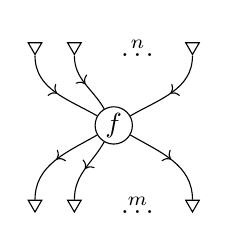
\begin{tikzpicture}
    \node[outer] (a1) at (-1,1) {};
    \node[outer] (a2) at (-.5,1) {};
    \node at (0.3,1) {$\overset{n}{\dots}$};
    \node[outer] (an) at (1,1) {};
    \node[vertex] (f) at (0,0) {$f$};
    \node[outer] (b1) at (-1,-1) {};
    \node[outer] (b2) at (-.5,-1) {};
    \node at (0.3,-1) {$\overset{m}{\dots}$};
    \node[outer] (bn) at (1,-1) {};
    \draw[edge] (a1) to[out=-90,in=150] (f);
    \draw[edge] (a2) to[out=-90,in=120] (f);
    \draw[edge] (an) to[out=-90,in=30] (f);
    \draw[edge] (f) to[out=-150,in=90] (b1);
    \draw[edge] (f) to[out=-120,in=90] (b2);
    \draw[edge] (f) to[out=-30,in=90] (bn);
  \end{tikzpicture}
\end{center}
This is an $(n,m)$-bracketed hypergraph with exactly one non-root vertex and with bracketings $n=\overbrace{1+1+\cdots+1}^n$ and $m=\overbrace{1+1+\cdots+1}^m$.
For any polygraph $P$, morphisms $(C_{n,m})_0 \to P$ are in bijection with vertices of $P$ having in-degree $n$ and out-degree $m$.

Now, for any polygraph $P$, we define $\eta_P : P \to T P$ as follows:
\begin{enumerate}
\item $\eta:P(0) \to TP(0)$ sends an object $x\in P(0)$ to its classifying map $x:\mathbf{1}\to P$, and similarly on arrows.
\item $\eta:P(n,m) \to TP(n,m)$ sends an object $f\in P(n,m)$ to its classifying map $f:(C_{n,m})_0\to P$, and similarly on arrows.
\end{enumerate}

\begin{thm}
  This defines a fully faithful cartesian 2-natural transformation $\eta: 1\to T$.
\end{thm}
\begin{proof}
  Naturality is easy, since postcomposing classifying maps is the same as acting on objects and arrows.
  Full faithfulness on $0$-parts is easy, while on $(n,m)$-parts it follows from the fact that $C_{n,m}$ has no nontrivial automorphisms.
  Finally, $\eta$ is cartesian, meaning that its naturality squares are pullbacks, since its image consists precisely of the objects and arrows involving $\mathbf{1}$ or $C_{n,m}$.
\end{proof}

Of course, there are many different (isomorphic) $(n,m)$-corollas.
However, the theorem is true as long as we fix a \emph{particular} such corolla for each $(n,m)$ to use in defining $\eta$.
The existence of other corollas means that $\eta$, though fully faithful, is not replete: objects of $TP$ defined using other corollas are isomorphic to ones in the image of $\eta$ but are not in the image of $\eta$ themselves.

Using insertion of hypergraphs, we define a cartesian 2-natural transformation $\mu:T^2\to T$.
\fxnote{Incomplete}

However, the monad laws hold only up to coherent isomorphism, so that we have a ``cartesian pseudomonad'' of a fairly strict sort (the functor and transformations are strict and strictly cartesian; only the monad laws are pseudo).
\fxnote{Incomplete}

\begin{defn}
  A $T$-pseudoalgebra is called a \textbf{double hypercategory}.
\end{defn}

A double hypercategory $H$ has the following structure:
\begin{itemize}
\item A set of \emph{objects}, the objects of the category $H(0)$.
\item A set of \emph{vertical arrows}, the arrows of $H(0)$, which can be composed in the usual way.
\item An (unbiased, non-strict) monoidal structure on the category of objects and vertical arrows.
\item For each $n,m$, a set of \emph{horizontal arrows} with lists of $n$ objects as source and $m$ objects as target (the objects of the category $H(n,m)$).
\item For each $n,m$, a set of \emph{2-cells} with horizontal arrows as ``vertical source and target'', and lists of $n$ vertical arrows and $m$ vertical arrows as ``horizontal source and target''.
  These can be composed vertically.
\item ``Horizontal composition'' operations on horizontal arrows and 2-cells, parametrized by bracketed hypergraphs.
  That is, if we label the non-root vertices of any rooted locally-ordered directed hypergraph by horizontal arrows of $H$, in such a way that the edges are labeled compatibly by objects, and bracket the incoming and outgoing edges to the root, then we obtain a composed horizontal arrow whose source and target are obtained by applying the monoidal structure on objects to the groups in the brackets.
  We can similarly compose hypergraphs labeled by 2-cells, and this operation is functorial with respect to vertical composition.
\item Moreover, isomorphisms of bracketed hypergraphs induce isomorphisms of composed horizontal arrows, naturally.
  In particular, this applies to \emph{automorphisms}.
\end{itemize}

\begin{defn}
  If a double hypercategory has only identity vertical arrows, we call it a \textbf{2-hypercategory}.
  If it additionally has only identity 2-cells, we call it a \textbf{hypercategory}.%
  \footnote{The word ``hypercategory'' was also used by~\cite{hmt:strict-n-hypercats,mt:omega-hypergraphs}.
    Our meaning is somewhat different, but not unrelated since they also use a kind of hypergraph.
    The ``hyperstructures'' of~\cite{baas:higher-structures} are also related, although in contrast to both of these references we consider here only one dimension of hyper-dependency.}
\end{defn}

\begin{eg}
  Let \bC be a symmetric monoidal category in which every object is equipped with the structure of a Frobenius algebra (but we do \emph{not} assume that all morphisms of \bC are monoid or comonoid homomorphisms).
  Then \bC has the structure of a hypercategory.
  In fact, it could be that this is exactly what a hypercategory is.
\end{eg}

\begin{eg}
  More generally, a sufficiently strictly monoidal 2-category in which every object has the structure of a Frobenius pseudomonoid~\cite{street:frob-psmon} gives rise to a 2-hypercategory.
  In particular, this applies to any cartesian bicategory~\cite{ckww:cartbicats-ii} in which every object is Frobenius~\cite{ww:frob-cart} and in which the monoidal structure is strict enough.

  In general, what can we take the vertical arrows to be?
  Arbitrary left adjoints?
  Morphisms that are colax for both monoid and comonoid structures?
\end{eg}

\begin{eg}
  If \bS has finite products, then an \bS-indexed monoidal category with indexed homotopy coproducts preserved by the tensor product on both sides, in the sense of~\cite{ps:indexed}, gives rise to a double hypercategory whose vertical category is \bS.
\end{eg}




\section{Virtual double hypercategories}
\label{sec:vdhc}

Our main purpose in defining the pseudomonad $T$ was to consider $T$-multicategories.
Leinster~\cite{leinster:higher-opds} defines $T$-multicategories with respect to a cartesian monad on any category with pullbacks.
Here we have only a pseudomonad on \cpg, but this causes little difficulty, especially since we are interested in the ``object-discrete'' case.

\begin{defn}
  A \textbf{virtual double hypercategory} $M$ consists of the following.
  \begin{enumerate}
  \item A polygraph $M_0$.
  \item A discrete fibration of \Cat-polygraphs $M_1 \to M_0 \times TM_0$.
  \item A composition operation $M_1 \times_{TM_0} TM_1 \to M_1$ over $1\times \mu$:
    \[
    \begin{tikzcd}
      M_1 \times_{TM_0} TM_1 \ar[r,dashed] \ar[d] & M_1\ar[d]\\
      M_0 \times TTM_0 \ar[r,"1\times \mu"'] & M_0\times TM_0.
    \end{tikzcd}
    \]
  \item A unit $M_0 \to M_1$ over $(1,\eta)$:
    \[
    \begin{tikzcd}
      M_0 \ar[r,dashed] \ar[d,equals] & M_1 \ar[d] \\
      M_0\ar[r,"{(1,\eta)}"'] & M_0\times TM_0.
    \end{tikzcd}
    \]
  \item An associativity isomorphism lying over the pseudomonad coherence isomorphism:
    \[\hspace{-2cm}
    \begin{tikzcd}
      & M_1 \times_{TM_0} TM_1 \ar[drr] \ar[ddd]\\
      M_1 \times_{TM_0} TM_1 \times_{TTM_0} TTM_1 \ar[ur] \ar[drr] \ar[ddd] \ar[rrr,phantom,"\cong"] &&&
      M_1 \ar[ddd] \\
      && M_1 \times_{TM_0} TM_1  \ar[ur]\ar[ddd]\\
      & M_0\times TTM_0\ar[drr] \\
      M_0 \times TTTM_0 \ar[ur] \ar[drr] \ar[rrr,phantom,"\cong"] &&&
      M_0\times TM_0 \\
      && M_0\times TTM_0\ar[ur]
    \end{tikzcd}\hspace{-2cm}
    \]
  \item Unit isomorphisms lying over the pseudomonad coherence isomorphisms:
    \[
    \begin{tikzcd}
      & M_1 \times_{TM_0} TM_1 \ar[dr] \ar[dddr,phantom,"\cong" very near start] \ar[dd] \\
      M_1 \ar[rr,equals] \ar[ur]\ar[dd] &~ & M_1\ar[dd]\\
      & M_0\times TM_0 \times TTM_0 \ar[dr] \ar[d,phantom,"\cong"] \\
      M_0\times TM_0 \ar[rr,equals]\ar[ur] &~& M_0\times TM_0
    \end{tikzcd}
    \]
    (There are two such isomorphisms, but the pictures look the same except that the omitted labels on the arrows should be different.)
  \end{enumerate}
\end{defn}

Since $M_1 \to M_0\times TM_0$ is assumed to be a discrete fibration, the coherence isomorphisms are unique, and automatically satisfy any axioms we might wish them to; thus we do not bother writing down those axioms (which would simply lift the corresponding pseudomonad axioms).
Explicitly, a virtual double hypercategory has the following structure.

\begin{enumerate}
\item A set of \emph{objects} (the objects of $M_0$).
\item A set of \emph{vertical multi-arrows}, with source a finite list of objects and target a single object (the objects of $M_1$).
  These can be composed as in an ordinary (non-symmetric) multicategory.
\item For each $n,m$, a set of \emph{horizontal arrows} with lists of $n$ objects as source and $m$ objects as target (the morphisms in the polygraph $M_0$).
\item A set of \emph{2-cells}, each of which has a bracketed hypergraph labeled by horizontal arrows as its vertical source, a single horizontal arrow as its vertical target, and lists of vertical multi-arrows as its horizontal source and target.
\item Each horizontal arrow has an identity 2-cell.
\item A composition operation on 2-cells that involves hypergraph insertion, which is appropriately associative and unital.
\end{enumerate}

We also have algebras over generalized multicategories, for which again we restrict to the discrete case.
Here there is no room for nontrivial isomorphisms at all.

\begin{defn}
  If $M$ is a virtual double hypercategory, an \textbf{$M$-algebra} consists of the following.
  \begin{enumerate}
  \item A polygraph $A$ with a map $A \to M_0$.
  \item An action map $M_1 \times_{TM_0} TA \to A$ over $M_0$.
  \item The action is associative and unital:
    \[\hspace{-2cm}
    \begin{tikzcd}
      M_1 \times_{TM_0} TM_1 \times_{TTM_0} TTA \ar[r] \ar[d] &M_1 \times_{TM_0} TA \ar[d]\\
      M_1 \times_{TM_0} TA \ar[r] & A
    \end{tikzcd}
    \qquad
    \begin{tikzcd}
      A \ar[r] \ar[dr,equals] & M_1 \times_{TM_0} TA\ar[d] \\ & A
    \end{tikzcd}\hspace{-2cm}
    \]
  \end{enumerate}
\end{defn}


\section{Undirected hypercategories and kits}
\label{sec:kits}

Can define similar monad using undirected hypergraphs.
The virtual undirected ones are a special case of directed virtual ones in which all sources are empty.
Kits should be a virtual undirected ones living over a ``shape'' one that marks variance.


\section{Type theory of virtual double hypercategories}
\label{sec:type-theory}

We adopt a ``type-theoretic rule'' notation for 2-cells in virtual double hypercategories.
To describe a labeled hypergraph, we assign a variable to each edge, and declare the variables as having the corresponding objects as ``types'' with their genera as annotations on the typing declaration, for instance
\begin{mathpar}
  x :^0 p \and y:^1 p \and z:^0 q
\end{mathpar}
where $p,q,r$ are objects of $M$.
In practice the genera will almost always be $0$, in which case we omit to notate them.
We notate the vertices as sequents with their labeling horizontal arrow as a term, and with their incident edges as the input and output variables:
\begin{mathpar}
  (x,y,x) \types \alpha: (x,z) \and
  (z,z,y) \types \beta:()
\end{mathpar}
Thus, we must have $\alpha:(p,p,p) \to (p,q)$ and $\beta : (q,q,p) \to ()$.
These declarations all occur in the ``premises''.
Finally, we treat vertical multi-arrows as function symbols and ``apply'' them to the variables denoting the corresponding edges, then place the resulting terms in a ``conclusion'' sequent, labeled again by a horizontal arrow:
\begin{mathpar}
  (F(x,y),x) \types \gamma : (z,G())
\end{mathpar}
For vertical identity arrows, we simply write the variable itself, i.e.\ $x$ means $1_p(x)$ and $z$ means $1_q(z)$.
If $F:(p,p)\to q$ and $G:() \to p$, then we must have $\gamma : (q,p) \to (q,p)$.
Putting the above examples together, we obtain the rule
\begin{mathpar}
  \inferrule{x :^0 p \\ y:^1 p \\ z:^0 q \\
    (x,y,x) \types \alpha: (x,z) \\ (z,z,y) \types \beta:()}
  {(F(x,y),x) \types \gamma : (z,G())}
\end{mathpar}
which corresponds to the following graphically drawn 2-cell:
\begin{center}
  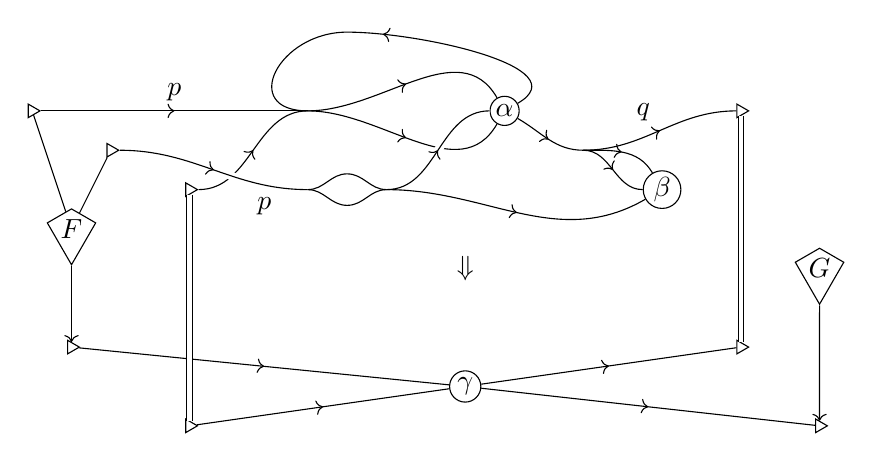
\begin{tikzpicture}
    \node[houter] (Fxy) at (.5,0) {};
    \node[houter] (idx) at (2,-1) {};
    \node[vertex] (gm) at (5.5,-.5) {$\gamma$};
    \node[houter] (idz) at (9,0) {};
    \node[houter] (G) at (10,-1) {};
    \draw[edge] (Fxy) -- (gm);
    \draw[edge] (idx) -- (gm);
    \draw[edge] (gm) -- (idz);
    \draw[edge] (gm) -- (G);
    \node[kite,draw,inner sep=1pt] (Gin) at (10,1) {$G$};
    \draw[->] (Gin) -- (G);
    \node[houter] (zout) at (9,3) {};
    \draw[double,double equal sign distance] (zout) -- (idz);
    \node[houter] (xin) at (2,2) {};
    \draw[double,double equal sign distance] (xin) -- (idx);
    \node[houter] (xyinx) at (0,3) {};
    \node[houter] (xyiny) at (1,2.5) {};
    \node[kite,draw,inner sep=1pt] (F) at (.5,1.5) {$F$};
    \draw (xyinx) -- (F);
    \draw (xyiny) -- (F);
    \draw[->] (F) -- (Fxy);
    \node[vertex] (be) at (8,2) {$\beta$};
    \node[vertex] (al) at (6,3) {$\alpha$};
    \coordinate (x) at (3.5,3);
    \coordinate (y) at (3.5,2);
    \draw[edge] (xyinx) to[out=0,in=180] node[auto] {$p$} (x);
    \draw[edge] (xin) to[out=0,in=180] (x);
    \draw[cross] (xyiny) to[out=0,in=180] (y);
    \draw[edge] (xyiny) to[out=0,in=180] node[auto,swap,very near end] {$p$} (y);
    \draw[edge] (x) to[out=0,in=120] (al);
    \draw[edge] (x) to[out=0,in=-120] (al);
    \coordinate (y2) at (4.5,2);
    \draw[cross] (y2) to[out=0,in=-180] (al);
    \draw[edge] (y2) to[out=0,in=-180] (al);
    \draw (y) to[out=0,in=180] (4,2.2) to[out=0,in=180] (y2);
    \draw (y) to[out=0,in=180] (4,1.8) to[out=0,in=180] (y2);
    \draw[edge] (al) to[out=30,in=0] (4,4) to[out=180,in=180,looseness=2] (x);
    \coordinate (z) at (7,2.5);
    \draw[edge] (al) to[out=-30,in=180] (z);
    \draw[edge] (z) to[out=0,in=120] (be);
    \draw[edge] (z) to[out=0,in=180] (be);
    \draw[edge] (y2) to[out=0,in=-150] (be);
    \draw[edge] (z) to[out=0,in=-180] node[auto] {$q$} (zout);
    \node at (5.5,1) {$\Downarrow$};
  \end{tikzpicture}
\end{center}

Identity 2-cells are easy:
\[ \inferrule{ (x,y,z) \types \alpha : (u,v,w) }{ (x,y,z) \types \alpha : (u,v,w) }\]
Composition of 2-cells is, thankfully, well-notated by combining rules in derivation trees, and \emph{substituting} the terms such as $F(x,y)$ in the conclusion of one rule into the variables occurring in the premises of another.
We do have to be careful that the vertical arrow parts match up between all the 2-cells we are precomposing with.
\fxnote{Some examples?}

It is important to note that when we write a 2-cell as a ``rule'' we are not ``deriving the conclusion from the premises''.
Instead each ``rule'' is a datum, namely the 2-cell, and putting together rules into derivation trees is an operation on these data.

When we get to \emph{$M$-algebras}, however, the rules become operations on sequents.
Here we notate the objects lying over an object $p$ by
\[A \type_p \qquad\text{or}\qquad A_p,\]
and the morphisms lying over $\alpha : (p,q,r) \to (u,v)$ by
\[(A_p,B_q,C_r) \types_\alpha f : (D_u,E_v).\]
Now the 2-cell considered above \emph{acts} on morphisms in the algebra, which we can interpret as a rule of the usual sort that produces a conclusion from the premises:
\begin{mathpar}
  \inferrule{A \type_p \\ B \type^1_p \\ C \type_q \\\\
    (A,B,A) \types_\alpha f : (A,C) \\ (C,C,B) \types_\beta g :()}
  {(F(A,B),A) \types_\gamma g\circ_\rho f : (C,G())}
\end{mathpar}
where $g\circ_\rho f$ denotes a sort of ``composition'' of $f$ and $g$ parametrized by the rule $\rho$.
Note that the vertical arrows $F$ and $G$ act similarly on \emph{types}, which we can notate with type formation rules:
\begin{mathpar}
  \inferrule{A\type_p \\ B\type_p}{F(A,B) \type_q}
  \and
  \inferrule{ }{G() \type_p}
\end{mathpar}

In this way, we can interpret a virtual double hypercategory as a reasonably general sort of \emph{specification of a sequent calculus}.
The objects are the \emph{modes} to which the types can belong.
The horizontal arrows are the \emph{mode morphisms}, or \emph{sequent forms}.
The vertical arrows are the \emph{type formation rules}.
And the 2-cells are the \emph{derivation rules} for sequents.
Each derivation rule takes as premises some number of types, each with a specified mode, and some number of sequents containing those types, each with a specified form, and yields as a conclusion a sequent with a specified form containing some of the types from the premises together with potentially other new types formed from them by the formation rules.
We call this a ``sequent calculus'' because the type formation operators can only appear in the conclusion; all types in the premises must be (meta-)variables.

Note that all the contraction, weakening, composition, and identities are performed formally in the vertical domain.
We contract two types by making the corresponding flags incident on the same edge, and so on.
In the type-theoretic notation, this is indicated by using the same (meta-)variable for the types in the corresponding places.
Even the symmetric action (exchange) is performed formally in the domain, since the incoming and outgoing edges on the root are ordered, and the vertical multi-arrows preserve ordering --- but this ordering is not visible in the premises of the type-theoretic notation, instead being indicated by the order in which the (meta-)variables appear in the conclusion.

The fact that vertical arrows and 2-cells have an algebraic structure of composition means that all \emph{derivable} rules are present on an equal footing with the primitive ones, along with all equations that hold between such derivations.
The primitive rules and primitive equality axioms between composites of these form a \emph{presentation} of a virtual double hypercategory by generators and relations.


\section{Examples}
\label{sec:examples}

For now, we consider only examples without type formation rules.

\subsection{Intuitionistic type theories}
\label{sec:intuitionistic}

We obtain intuitionistic type theories simply by requiring all mode morphisms to have unary targets.
If we have one mode $p$ and one such morphism $p^n \to p$ for each $n$, we can express the identity and cut rules of ordered logic:
\begin{mathpar}
  \inferrule{A\type}{A\types A}
  \and
  \inferrule{\Gamma\types A \\ \Delta,A,\Psi\types B}{\Delta,\Gamma,\Psi\types B}
\end{mathpar}
We can assert axioms on the composites of these to obtain the semantic structure of a non-symmetric multicategory.

We can then add the exchange rule of intuitionistic linear logic:
\begin{mathpar}
  \inferrule{\Gamma,A,B,\Delta\types C}{\Gamma,B,A,\Delta\types C}
\end{mathpar}
with axioms yielding a symmetric multicategory.


\bibliography{../all.bib}
\bibliographystyle{alpha}

\end{document}
